\documentclass{beamer}
\usepackage{mathrsfs,xcolor,setspace,comment,centernot,listings,framed,subfig,ragged2e}
\usepackage[utf8]{inputenc}
\usepackage[T1]{fontenc}

\DeclareMathOperator{\Cov}{Cov}
\DeclareMathOperator{\Var}{Var}
\DeclareMathOperator{\E}{\mathbb{E}}
\DeclareMathOperator{\Proba}{\mathbb{P}}

\newcommand{\Covb}[2]{\ensuremath{\Cov\!\left[#1,#2\right]}}
\newcommand{\Eb}[1]{\ensuremath{\E\!\left[#1\right]}}
\newcommand{\Pb}[1]{\ensuremath{\Proba\!\left[#1\right]}}
\newcommand{\Varb}[1]{\ensuremath{\Var\!\left[#1\right]}}

% norm
\newcommand{\norm}[1]{\| #1 \|}

\newcommand{\indep}{\rotatebox[origin=c]{90}{$\models$}}



% config du theme metropolis
\usetheme[progressbar=frametitle,block=fill, titleformat=smallcaps,sectionpage=progressbar,]{metropolis}


\title{A generic and modular simulation model for suburban densification}
\subtitle{}

\date{11/03/2025\\
\textit{Journée de la Recherche UGE-IGN-ENSG 2025}\\
Session: Simulating Social and Spatial Processes}

\author{Juste Raimbault\textsuperscript{1,2,3,4}, Vera Götze\textsuperscript{1} and Julien Perret\textsuperscript{1,5}}
\institute{\textsuperscript{1}LaSTIG, IGN-ENSG-UGE\\
\textsuperscript{2}CASA, UCL\\
\textsuperscript{3}UPS CNRS 3611 ISC-PIF\\
\textsuperscript{4}UMR CNRS 8504 Géographie-cités\\
\textsuperscript{5}LaDéHiS, EHESS
}



%definition de la couleur du texte dans la balise \alert{}
\definecolor{vertIGN}{HTML}{96C31E} % vert IGN %vrai valeur #97BE0D
\setbeamercolor{alerted text}{fg=vertIGN}

\definecolor{grisIGN}{HTML}{22292F} % Gris IGN tiré vers le noir 
\setbeamercolor{background canvas}{bg=grisIGN}


% code pour placer le log ENSG dans le bandeau de titre 
\makeatletter
\setbeamertemplate{frametitle}{%
  \nointerlineskip%
  \begin{beamercolorbox}[%
      wd=\paperwidth,%
      sep=0pt,%
      leftskip=\metropolis@frametitle@padding,%
      rightskip=\metropolis@frametitle@padding,%
    ]{frametitle}%
  \metropolis@frametitlestrut@start%
  \insertframetitle%
  \nolinebreak%
  \metropolis@frametitlestrut@end%
  \hfill
  \raisebox{-0.6ex}{
\includegraphics[height=4ex,keepaspectratio]{figures/logoENSG_small.jpg}}
  \end{beamercolorbox}%
}


\newcommand{\noun}[1]{\textsc{#1}}
\newcommand{\jitem}[1]{\item \begin{justify} #1 \end{justify} \vfill{}}
\newcommand{\sframe}[2]{\frame{\frametitle{#1} #2}}

\newenvironment{centercolumns}{\begin{columns}[c]}{\end{columns}}
%\newenvironment{jitem}{\begin{justify}\begin{itemize}}{\end{itemize}\end{justify}}



\usepackage{pifont}
\newcommand{\cmark}{\ding{51}}
\newcommand{\xmark}{\ding{55}}


\usepackage{multirow}

\makeatother




% logo ENSG première page 
\titlegraphic{\vspace{4cm}\flushright
\includegraphics[width=2cm,height=2cm]{figures/logoENSG_big.png}} 





\begin{document}
\metroset{background=dark} % change background theme according to manual
\maketitle	



%  Suburban densification is a process important for urban sustainability, for example to limit urban sprawl and increase public transport ridership. Its dynamics remain difficult to grasp as many stakeholders at different scales are involved, from home and land owners to developpers and public authorities. They furthermore can change drastically with the context and country. We propose in this contribution a formal description of an agent-based simulation model, aimed at capturing such processes with enough genericity to be applied across 3 European countries (France, UK and Germany, studied in the context of the Subdense research project). The modular architecture allows including submodels for specific computations, such as the SimPLU3d model for densification potential and the ParcelManager model for land division. We expect this first proposal to be refined after its application to case studies and its calibration on empirical data, and a discussion with qualitative researchers working with densification stakeholders.

\sframe{Context: the SUBDENSE project}{

\medskip

\begin{columns}
	\begin{column}{0.6\textwidth}
		The SubDense European project studies the dynamics of suburban densification by:
 
	\end{column}
	\begin{column}{0.4\textwidth}
		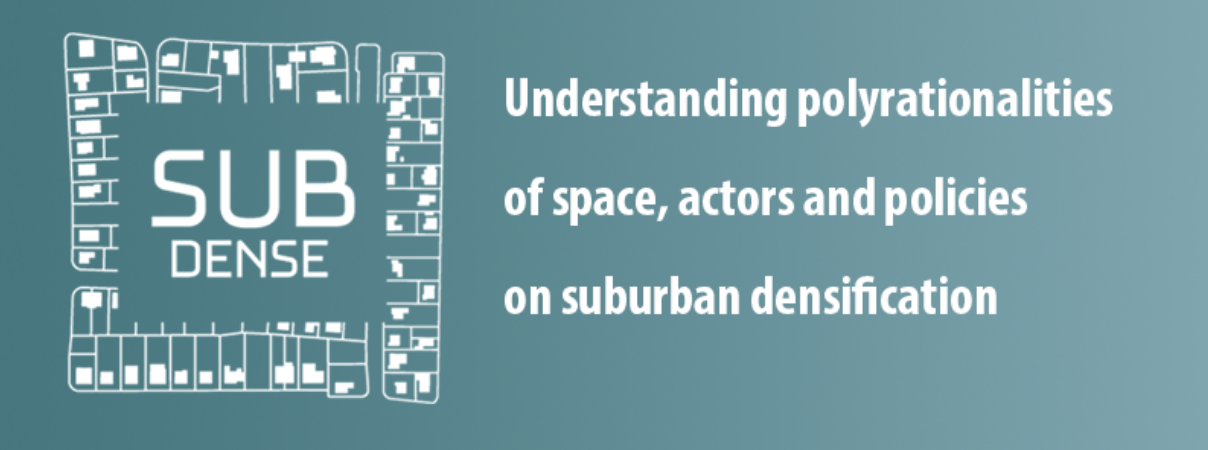
\includegraphics[height=0.2\textheight]{figures/subdense.png}
	\end{column}
\end{columns}


\begin{itemize} 
	\item exploring how diverse strategies of land policy interact with landowners’ and local stakeholders’ interest and agency to shape suburban densification and their impact on suburbia across different planning systems (France, Germany, UK);
	\item combining quantitative approaches (geodata analysis and geosimulation) with qualitative approaches (social and policy science and planning).
\end{itemize}

\bigskip

\centering


\includegraphics[height=0.1\textheight]{figures/logos.png}

\includegraphics[height=0.1\textheight]{figures/tud.png}


}

\sframe{A collaborative dashboard}{


% Change detection



}




\sframe{Research objective}{

% WP3 and obejctive of the ABM

}


\sframe{Simulating urban densification}{

% literature

% \cite{burke20243d} residents, developers, landowners, and the local zoning authority 

% \cite{leao2018agent} parcels and buildings as autonomous agents

% \cite{pawar2023analysis} data driven abm of household relocation and impact on density

% \cite{chakraborty2022cellular} CA models to model and predict



}





\sframe{Model description following the ODD protocol}{

\cite{grimm2020odd}

\centering

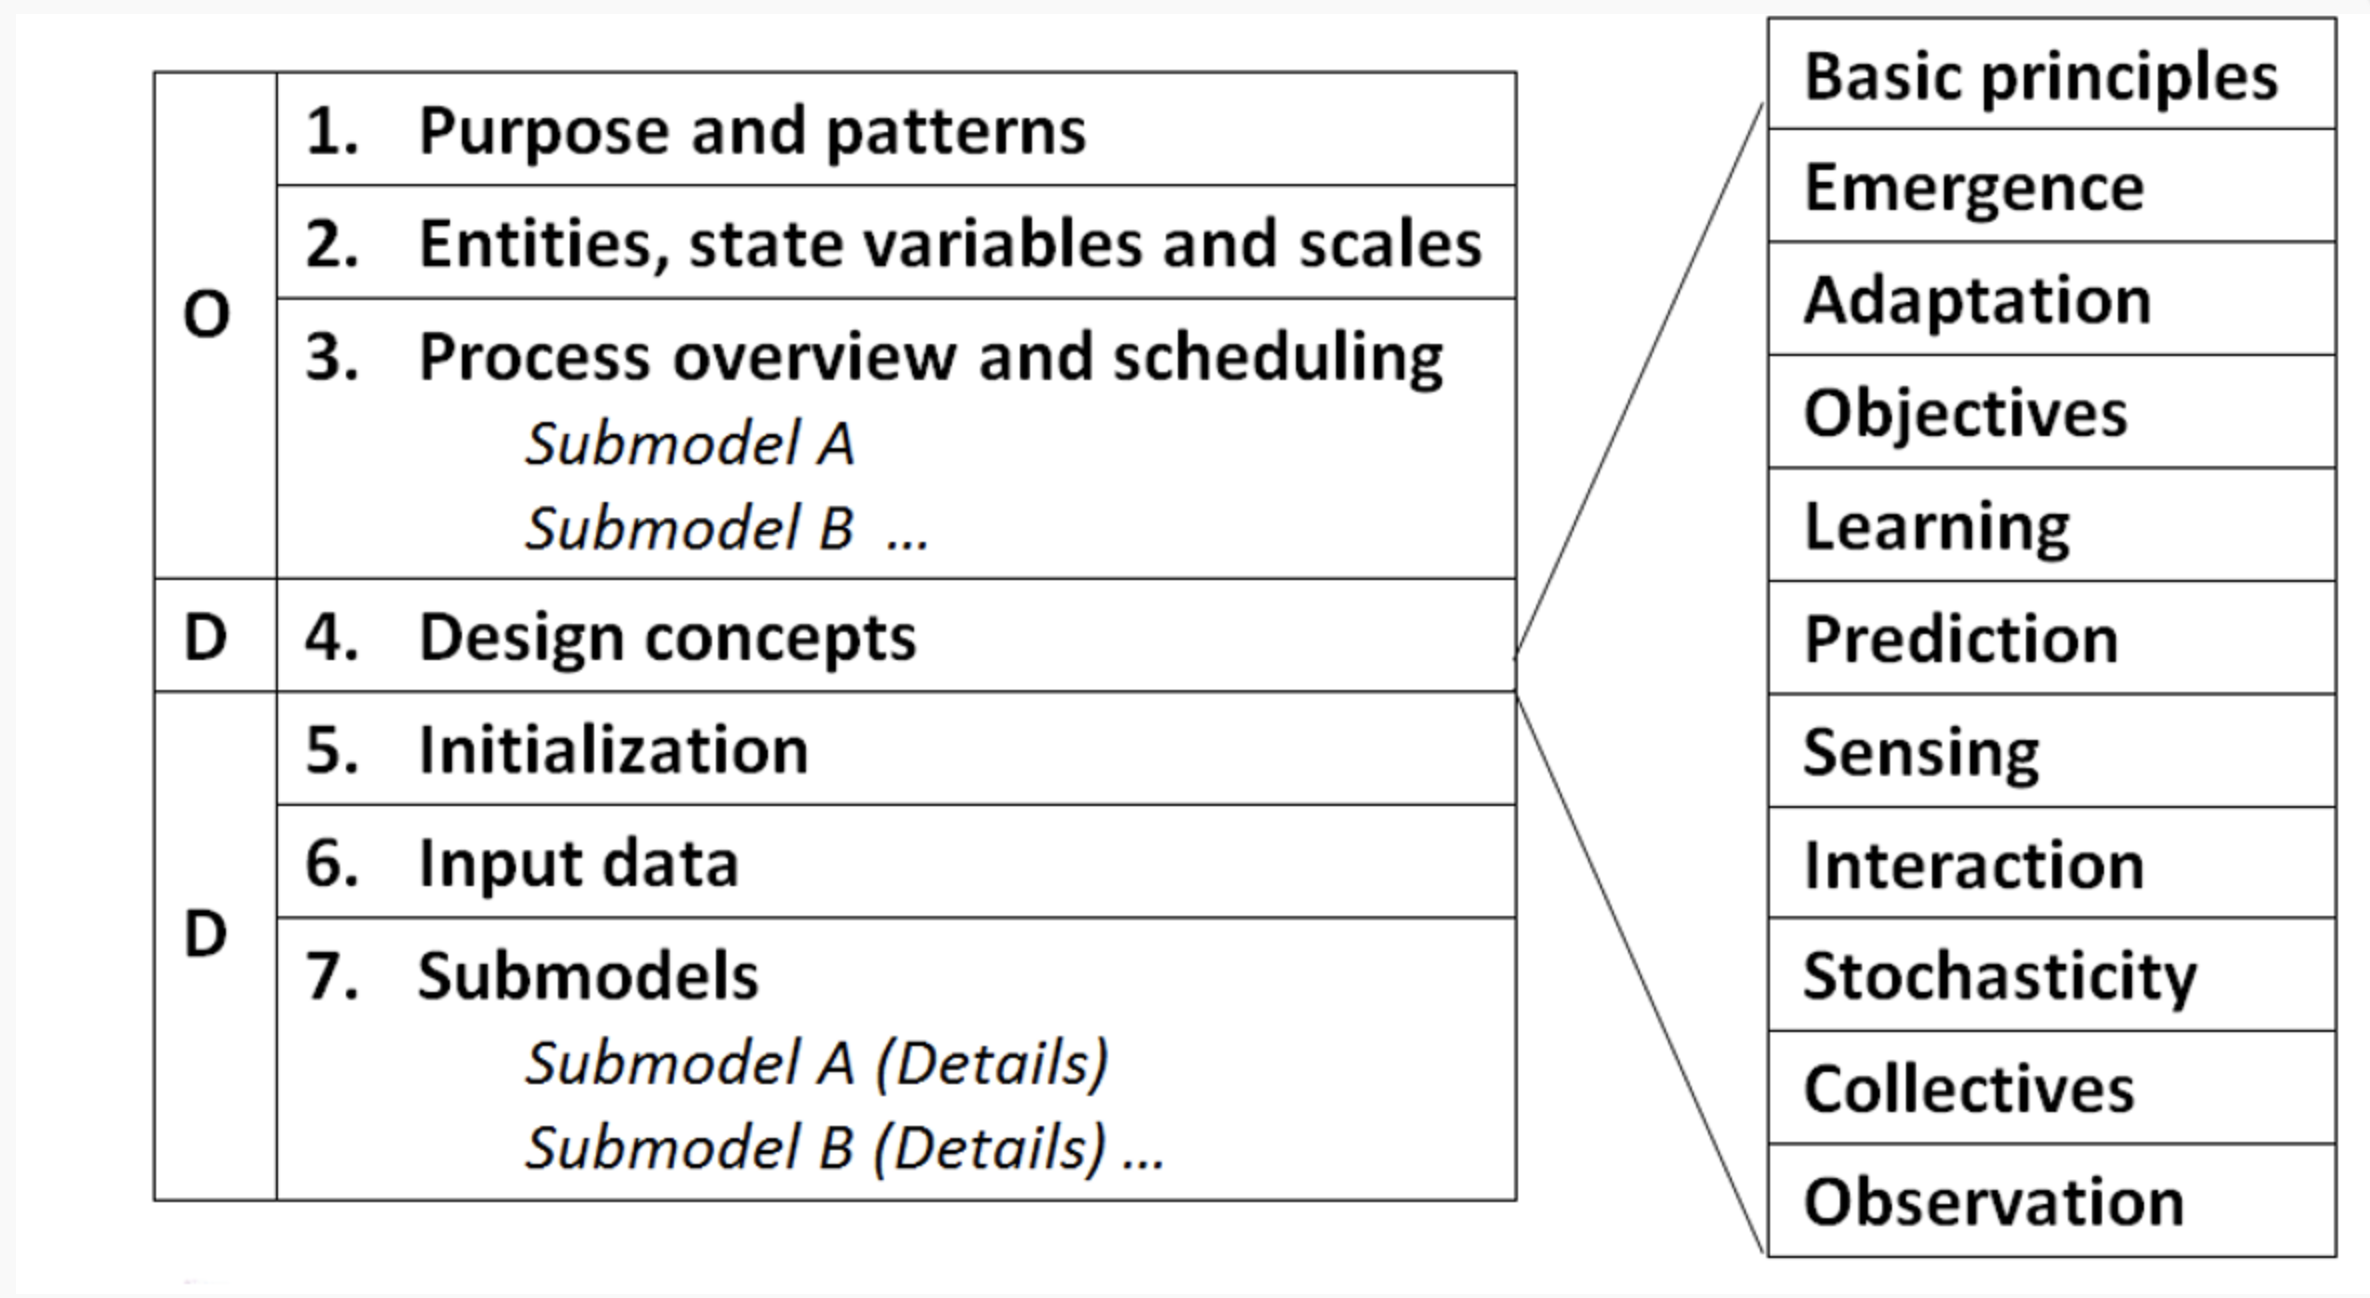
\includegraphics[width=0.8\textwidth]{figures/odd.png}

}

\sframe{Overview}{

}

\sframe{Design concepts}{

}

\sframe{Details}{

}

\sframe{The SimPLU model for densification potential}{

}


\sframe{The ParcelManager model to split parcels}{

}


\sframe{Open issues and next steps}{

}


%%%%%%%%%%%%%%%%%%%%%
\begin{frame}[allowframebreaks]
\frametitle{References}
\bibliographystyle{apalike}
\bibliography{biblio}
\end{frame}
%%%%%%%%%%%%%%%%%%%%%%%%%%%%





\end{document}

